% !TEX TS-program = xelatex
% !BIB program = bibtex
% !TeX spellcheck = ru_RU
% !TEX root = talk.tex

\documentclass
  [ russian
  , aspectratio=1610 % Для защит онлайн лучше использовать разрешение не 4х3
  ] {beamer}


%%% PDF settings
\pdfvariable minorversion 7 % Set PDF version to 1.7.

%%% Fonts and language setup.
\usepackage{polyglossia}
% Setup fonts.
\usepackage{fontspec}
\setmainfont{CMU Serif}
\setsansfont{CMU Sans Serif}
\setmonofont{CMU Typewriter Text}

\usepackage{microtype} % Add fancy-schmancy font tricks

\usepackage{xcolor} % Add colors support.

%% Math
\usepackage{amsmath, amsfonts, amssymb, amsthm, mathtools} % Advanced math tools.
\usepackage{thmtools}
\usepackage{unicode-math} % Allow TTF and OTF fonts in math and allow direct typing unicode math characters.
\unimathsetup{
    warnings-off={
            mathtools-colon,
            mathtools-overbracket
        }
}
\setmathfont{Latin Modern Math} % default
\setmathfont[range={\setminus,\varnothing,\smashtimes}]{Asana Math}

%%% Images
\usepackage{graphicx}
\graphicspath{{figures/}}
\usepackage{import}

%%% Polyglossia setup after (nearly) everything as described in documentation.
\setdefaultlanguage{russian}
\setotherlanguage{english}

\usepackage{csquotes}

%%% Custom commands
\newcommand{\R}{\mathbb{R}}
\newcommand{\N}{\mathbb{N}}
\newcommand{\Z}{\mathbb{Z}}
\newcommand{\Q}{\mathbb{Q}}
\newcommand{\C}{\mathbb{C}}
\newcommand{\id}{\mathrm{id}}
\AtBeginDocument{\renewcommand{\leq}{\leqslant}}
\AtBeginDocument{\renewcommand{\geq}{\geqslant}}
\AtBeginDocument{\renewcommand{\Re}{\operatorname{Re}}}
\AtBeginDocument{\renewcommand{\Im}{\operatorname{Im}}}
\AtBeginDocument{\renewcommand{\phi}{\varphi}}
\AtBeginDocument{\renewcommand{\epsilon}{\varepsilon}}

%%% theorem-like envs
\theoremstyle{definition}

\declaretheoremstyle[spaceabove=0.5\topsep,
    spacebelow=0.5\topsep,
    headfont=\bfseries\sffamily,
    bodyfont=\normalfont,
    headpunct=.,
    postheadspace=5pt plus 1pt minus 1pt]{myStyle}
\declaretheoremstyle[spacebelow=\topsep,
    headfont=\bfseries\sffamily,
    bodyfont=\normalfont,
    headpunct=.,
    postheadspace=5pt plus 1pt minus 1pt,]{myStyleWithFrame}
\declaretheoremstyle[spacebelow=\topsep,
    headfont=\bfseries\sffamily,
    bodyfont=\normalfont,
    headpunct=.,
    postheadspace=5pt plus 1pt minus 1pt,
    qed=\blacksquare]{myProofStyleWithFrame}

\usepackage[breakable]{tcolorbox}
\tcbset{sharp corners=all, colback=white}
% \tcolorboxenvironment{theorem}{}
% \tcolorboxenvironment{theorem*}{}
% \tcolorboxenvironment{axiom}{}
% \tcolorboxenvironment{assertion}{}
% \tcolorboxenvironment{lemma}{}
% \tcolorboxenvironment{proposition}{}
% \tcolorboxenvironment{corollary}{}
% \tcolorboxenvironment{definition}{}
% \tcolorboxenvironment{proofReplace}{toprule=0mm,bottomrule=0mm,rightrule=0mm, colback=white, breakable }

\declaretheorem[name=Теорема, style=myStyleWithFrame]{theorem}
\declaretheorem[name=Теорема, numbered=no, style=myStyleWithFrame]{theorem*}
\declaretheorem[name=Аксиома, sibling=theorem, style=myStyleWithFrame]{axiom}
\declaretheorem[name=Преположение, sibling=theorem, style=myStyleWithFrame]{assertion}
\declaretheorem[name=Лемма, style=myStyleWithFrame]{lemma}
\declaretheorem[name=Предложение, sibling=theorem, style=myStyleWithFrame]{proposition}
\declaretheorem[name=Следствие, numberwithin=theorem, style=myStyleWithFrame]{corollary}

\declaretheorem[name=Определение, style=myStyleWithFrame]{definition}
\declaretheorem[name=Свойство, style=myStyle]{property}
\declaretheorem[name=Свойства, numbered=no, style=myStyle]{propertylist}

\declaretheorem[name=Пример, style=myStyle]{example}
\declaretheorem[name=Замечание, numbered=no, style=myStyle]{remark}

\declaretheorem[name=Доказательство, numbered=no, style=myProofStyleWithFrame]{proofReplace}
\renewenvironment{proof}[1][\proofname]{\begin{proofReplace}}{\end{proofReplace}}
% \declaretheorem[name=Доказательство, numbered=no, style=myProofStyleWithFrame]{longProof}

%%% Memoir settings
\chapterstyle{ger}
\setlength{\headheight}{2\baselineskip}

%%% HyperRef
\usepackage{hyperref}

\makeatletter

%!TEX root = vkr.tex

%% Параметры заполнения титульного листа
\usepackage{xkeyval}

%% Русскоязычный вариант
\define@key[ru]{mytitle}{chair}{\def\my@title@chair@ru{#1}}
\define@key[ru]{mytitle}{title}{\def\my@title@title@ru{#1}}
\define@key[ru]{mytitle}{group}{\def\my@title@group@ru{#1}}
\define@key[ru]{mytitle}{author}{\def\my@title@author@ru{#1}}
\define@key[ru]{mytitle}{supervisor}{\def\my@title@supervisor@ru{#1}}
\define@key[ru]{mytitle}{supervisorPosition}{\def\my@title@supervisorPosition@ru{#1}}
\define@key[ru]{mytitle}{reviewer}{\def\my@title@reviewer@ru{#1}}
\define@key[ru]{mytitle}{reviewerPosition}{\def\my@title@reviewerPosition@ru{#1}}
\define@key[ru]{mytitle}{consultant}{\def\my@title@consultant@ru{#1}}
\define@key[ru]{mytitle}{consultantPosition}{\def\my@title@consultantPosition@ru{#1}}
\define@key[ru]{mytitle}{year}{\def\my@title@year@ru{#1}}
\define@key[ru]{mytitle}{specialty}{\def\my@title@specialty@ru{#1}}
\define@key[ru]{mytitle}{programme}{\def\my@title@programme@ru{#1}}
\define@key[ru]{mytitle}{profile}{\def\my@title@profile@ru{#1}}
\define@choicekey*[ru]{mytitle}{type}{coursework,practice,prediploma,master,bachelor,production}{\def\my@title@type@ru{#1}}
\define@choicekey*[ru]{mytitle}{kind}{solution,experiment,production,comparison,theoretical}{\def\my@title@kind@ru{#1}}

%% Англоязычный вариант
\define@key[en]{mytitle}{chair}{\def\my@title@chair@en{#1}}
\define@key[en]{mytitle}{title}{\def\my@title@title@en{#1}}
\define@key[en]{mytitle}{group}{\def\my@title@group@en{#1}}
\define@key[en]{mytitle}{author}{\def\my@title@author@en{#1}}
\define@key[en]{mytitle}{supervisor}{\def\my@title@supervisor@en{#1}}
\define@key[en]{mytitle}{supervisorPosition}{\def\my@title@supervisorPosition@en{#1}}
\define@key[en]{mytitle}{reviewer}{\def\my@title@reviewer@en{#1}}
\define@key[en]{mytitle}{reviewerPosition}{\def\my@title@reviewerPosition@en{#1}}
\define@key[en]{mytitle}{consultant}{\def\my@title@consultant@en{#1}}
\define@key[en]{mytitle}{consultantPosition}{\def\my@title@consultantPosition@en{#1}}
\define@key[en]{mytitle}{year}{\def\my@title@year@en{#1}}
\define@key[en]{mytitle}{specialty}{\def\my@title@specialty@en{#1}}
\define@key[en]{mytitle}{programme}{\def\my@title@programme@en{#1}}
\define@key[en]{mytitle}{profile}{\def\my@title@profile@en{#1}}
\define@choicekey*[en]{mytitle}{type}{coursework,practice,prediploma,master,bachelor}{\def\my@title@type@en{#1}}
\define@choicekey*[en]{mytitle}{kind}{solution,experiment,production,comparison,theoretical}{\def\my@title@kind@en{#1}}

\newcommand{\filltitle}[2]{
    %% Значения по умолчанию для обоих языков
    \ifthenelse{\equal{#1}{ru}}
    {
        \presetkeys[#1]{mytitle}{
            year = {\the\year},
            type = {practice},
            reviewer = {},
            consultant = {},
            profile = {}
        }{}
    }
    {}
    \ifthenelse{\equal{#1}{en}}
    {
        \presetkeys[#1]{mytitle}{
            year = {\the\year},
            type = {practice},
            reviewer = {},
            consultant = {},
            profile = {}
        }{}
    }
    {}
    \setkeys[#1]{mytitle}{#2}
}


% !TeX spellcheck = ru_RU
% !TEX root = vkr.tex

%% Если что-то забыли, при компиляции будут ошибки Undefined control sequence \my@title@<что забыли>@ru
%% Если англоязычная титульная страница не нужна, то ее можно просто удалить.
\filltitle{ru}{
	%% Актуально только для курсовых/практик. ВКР защищаются не на кафедре а в ГЭК по направлению,
	%%   и к моменту защиты вы будете уже не в группе.
	chair              = {Кафедра системного программирования},
	group              = {21.Б10-мм},
	%
	%% Макрос filltitle ненавидит пустые строки, поэтому обязателен хотя бы символ комментария на строке
	%% Актуально всем.
	title              = {Разработка инфраструктуры для сборки проектов с открытым исходным кодом для архитектуры \riscv{}},
	%
	%% Здесь указывается тип работы. Возможные значения:
	%%   production - производственная практика;
	%%   coursework - отчёт по курсовой работе;
	%%   practice - отчёт по учебной практике;
	%%   prediploma - отчёт по преддипломной практике;
	%%   master - ВКР магистра;
	%%   bachelor - ВКР бакалавра.
	type               = {practice},
	%
	%% Здесь указывается вид работы. От вида работы зависят критерии оценивания.
	%%   solution - <<Решение>>. Обучающемуся поручили найти способ решения проблемы в области разработки программного обеспечения или теоретической информатики с учётом набора ограничений.
	%%   experiment - <<Эксперимент>>. Обучающемуся поручили изучить возможности, достоинства и недостатки новой технологии, платформы, языка и т. д. на примере какой-то задачи.
	%%   production - <<Производственное задание>>. Автору поручили реализовать потенциально полезное программное обеспечение.
	%%   comparison - <<Сравнение>>. Обучающемуся поручили сравнить несколько существующих продуктов и/или подходов.
	%%   theoretical - <<Теоретическое исследование>>. Автору поручили доказать какое-то утверждение, исследовать свойства алгоритма и т.п., при этом не требуя написания кода.
	kind               = {experiment},
	%
	author             = {Пономарев Николай Алексеевич},
	%
	%% Актуально только для ВКР. Указывается код и название направления подготовки. Типичные примеры:
	%%   02.03.03 <<Математическое обеспечение и администрирование информационных систем>>
	%%   02.04.03 <<Математическое обеспечение и администрирование информационных систем>>
	%%   09.03.04 <<Программная инженерия>>
	%%   09.04.04 <<Программная инженерия>>
	%% Те, что с 03 в середине --- бакалавриат, с 04 --- магистратура.
	specialty          = {02.03.03 <<Математическое обеспечение и администрирование информационных систем>>},
	%
	%% Актуально только для ВКР. Указывается шифр и название образовательной программы. Типичные примеры:
	%%   СВ.5006.2017 <<Математическое обеспечение и администрирование информационных систем>>
	%%   СВ.5162.2020 <<Технологии программирования>>
	%%   СВ.5080.2017 <<Программная инженерия>>
	%%   ВМ.5665.2019 <<Математическое обеспечение и администрирование информационных систем>>
	%%   ВМ.5666.2019 <<Программная инженерия>>
	%% Шифр и название программы можно посмотреть в учебном плане, по которому вы учитесь.
	%% СВ.* --- бакалавриат, ВМ.* --- магистратура. В конце --- год поступления (не обязательно ваш, если вы были в академе/вылетали).
	programme          = {СВ.5006.2019 <<Математическое обеспечение и администрирование информационных систем>>},
	%
	%% Актуально только для ВКР, только для матобеса и только 2017-2018 годов поступления. Указывается профиль подготовки, на котором вы учитесь.
	%% Названия профилей можно найти в учебном плане в списке дисциплин по выбору. На каком именно вы, вам должны были сказать после второго курса (можно уточнить в студотделе).
	%% Вот возможные вариканты:
	%%   Математические основы информатики
	%%   Информационные системы и базы данных
	%%   Параллельное программирование
	%%   Системное программирование
	%%   Технология программирования
	%%   Администрирование информационных систем
	%%   Реинжиниринг программного обеспечения
	% profile            = {Системное программирование},
	%
	%% Актуально всем.
	%supervisorPosition = {проф. каф. СП, д.ф.-м.н., проф.}, % Терехов А.Н.
	supervisorPosition = {старший преподаватель Кафедры\\системного программирования}, % Григорьев С.В.
	supervisor         = {Я.~А.~Кириленко},
	%
	%% Актуально только для практик и курсовых. Если консультанта нет, закомментировать или удалить вовсе.
	% consultantPosition = {должность ООО <<Место работы>>, степень,},
	% consultant         = {К.~К.~Консультант},
	%
	%% Актуально только для ВКР.
	% reviewerPosition   = {должность ООО <<Место работы>> степень},
	% reviewer           = {Р.~Р.~Рецензент},
}

% \filltitle{en}{
%     chair              = {Advisor's chair},
%     group              = {ХХ.BХХ-mm},
%     title              = {Template for SPbU qualification works},
%     type               = {practice},
%     author             = {FirstName Surname},
%     %
%     %% Possible choices:
%     %%   02.03.03 <<Software and Administration of Information Systems>>
%     %%   02.04.03 <<Software and Administration of Information Systems>>
%     %%   09.03.04 <<Software Engineering>>
%     %%   09.04.04 <<Software Engineering>>
%     %% Те, что с 03 в середине --- бакалавриат, с 04 --- магистратура.
%     specialty          = {02.03.03 ``Software and Administration of Information Systems''},
%     %
%     %% Possible choices:
%     %%   СВ.5006.2017 <<Software and Administration of Information Systems>>
%     %%   СВ.5162.2020 <<Programming Technologies>>
%     %%   СВ.5080.2017 <<Software Engineering>>
%     %%   ВМ.5665.2019 <<Software and Administration of Information Systems>>
%     %%   ВМ.5666.2019 <<Software Engineering>>
%     programme          = {СВ.5006.2019 ``Software and Administration of Information Systems''},
%     %
%     %% Possible choices:
%     %%   Mathematical Foundations of Informatics
%     %%   Information Systems and Databases
%     %%   Parallel Programming
%     %%   System Programming
%     %%   Programming Technology
%     %%   Information Systems Administration
%     %%   Software Reengineering
%     % profile            = {Software Engineering},
%     %
%     %% Note that common title translations are:
%     %%   кандидат наук --- C.Sc. (NOT Ph.D.)
%     %%   доктор ... наук --- Sc.D.
%     %%   доцент --- docent (NOT assistant/associate prof.)
%     %%   профессор --- prof.
%     supervisorPosition = {Sc.D, prof.},
%     supervisor         = {S.S. Supervisor},
%     %
%     consultantPosition = {position at ``Company'', degree if present},
%     consultant         = {C.C. Consultant},
%     %
%     reviewerPosition   = {position at ``Company'', degree if present},
%     reviewer           = {R.R. Reviewer},
% }


\newcommand{\academicGroup}{\my@title@group@ru}
\newcommand{\advisorChair}{\my@title@chair@ru}
% То, что в квадратных скобках, отображается внизу по центру каждого слайда.
\title[Короткое название]{\my@title@title@ru}
% То, что в квадратных скобках, отображается в левом нижнем углу.
\author[\my@title@author@ru]{\my@title@author@ru, группа \academicGroup}
\institute[СПбГУ]{}
\date[9 сентября 2024 г.]{}
\newcommand{\supervisor}{\my@title@supervisor@ru}
\newcommand{\supervisorPosition}{\my@title@supervisorPosition@ru}
\newcommand{\consultant}{\my@title@consultant@ru}
\newcommand{\consultantPosition}{\my@title@consultantPosition@ru}
\newcommand{\reviewer}{\my@title@reviewer@ru}
\newcommand{\reviewerPosition}{\my@title@reviewerPosition@ru}
\newcommand{\defenseYear}{\my@title@year@ru}

\makeatother
\begin{document}
{
\setbeamertemplate{footline}{}
% Лого университета или организации, отображается в шапке титульного листа
\begin{frame}
    
\includegraphics[width=1.4cm]{figures/SPbGU_Logo.png}
    \vspace{-35pt}
    \hspace{-10pt}
    \begin{center}
        \begin{tabular}{c}
            \scriptsize{Санкт-Петербургский государственный университет} \\
            \scriptsize{\advisorChair}
        \end{tabular}
        \titlepage
    \end{center}

    \btVFill

    {\scriptsize
        % У научного руководителя должна быть указана научная степень
        \textbf{Научный руководитель:}  \supervisorPosition~\supervisor \\
        % Консультанта может и не быть. Должна быть указана должность или ученая степень
        \textbf{Консультант:}  \consultantPosition~\consultant \\
        % Для учебной практики не обязателен. Должна быть указана должность или ученая степень
        \textbf{Рецензент:} \reviewerPosition~\reviewer \\
        % TODO: добавить условие на включение рецензента в зависимости от вида отчета
    }
    \makeatother
    \begin{center}
        \vspace{5pt}
        \scriptsize{Санкт-Петербург\\ \defenseYear}
    \end{center}
\end{frame}
}

\begin{frame}{Введение}
    \begin{itemize}
        \item Краткий обзор тематики работы (как вариант~--- устно, пока показывается титульный слайд)
        \item Не нужно определять общеизвестные понятия
        \item Применимость/полезность данной работы, обоснование выбора именно этой темы
        \item Если тема похожа на темы других работ (в том числе прошлых лет), надо явно описать разницу
    \end{itemize}
\end{frame}

\begin{frame}
    \frametitle{Существующие решения (инструменты, подходы, алгоритмы)}
    \begin{itemize}
        \item Перечислить инструменты/подходы, применяемые в области
        \item Указать их преимущества и недостатки (критика существующих решений/подходов)
    \end{itemize}

\end{frame}

\begin{frame}
    \frametitle{Существующие решения}
    Возможно, предметная область сложна и потребуется больше одного слайда, но затягивать введение не стоит. Постарайтесь уложиться в 1--2 слайда
    \begin{itemize}
        \item Выводы
              \begin{itemize}
                  \item Подвести итог
                  \item Указать недостатки существующих подходов, на борьбу с которыми
                        направленна данная работа
                  \item Чётко сформулировать существующую проблему, которая будет решаться в данной работе
              \end{itemize}
    \end{itemize}
\end{frame}

% Обязательный слайд: четкая формулировка цели данной работы и постановка задачи
% Описание выносимых на защиту результатов, процесса или особенностей их достижения и т.д.
\begin{frame}
    \frametitle{Постановка задачи}
    \textbf{Целью} работы является решение какой-то проблемы %озвученной выше
    \vspace{1em}

    \textbf{Задачи}:
    \begin{itemize}
        \item Выбрать алгоритм, подход, метод %основываясь на проведённом анализе проблемы, области, существующих решений
        \item Разработать алгоритм, делающий то-то с тем-то
        \item Доказать корректность алгоритма
        \item Реализовать предложенный алгоритм
        \item Провести экспериментальное исследование предложенной реализации
    \end{itemize}
\end{frame}

%Идеально, если есть по одному слайду на каждую поставленную задачу

\begin{frame}
    \frametitle{Алгоритм ABC\footnote{Результаты и обоснования выбора пути достижения цели}}
    За основу решения взят алгоритм ABC
    \begin{itemize}
        \item Почему именно он, а не другие
        \item Ключевые особенности выбранного алгоритма, важные для решения поставленных задач
    \end{itemize}
\end{frame}

% TODO(Kakadu): lstlisting will be better
\defverbatim[colored]{\CodeExample}{
    \begin{Verbatim}[commandchars=\\\{\}]
        \textcolor{blue}{string} res = \textcolor{orange}{""};
        \textcolor{blue}{for}(i = 0; i < l; i++) \{
        res = \textcolor{orange}{"()"} + res;
        \}
    \end{Verbatim}
}

\begin{frame}%[fragile]
    \frametitle{Новый алгоритм}
    \framesubtitle{Иллюстративные возможности: таблицы, картинки, код}
    % Задается ширина столбцов
    \begin{columns}[T]
        \begin{column}[t]{.4\textwidth}
            \begin{minipage}{2in} \CodeExample         \end{minipage}
            Аппроксимация:\\
            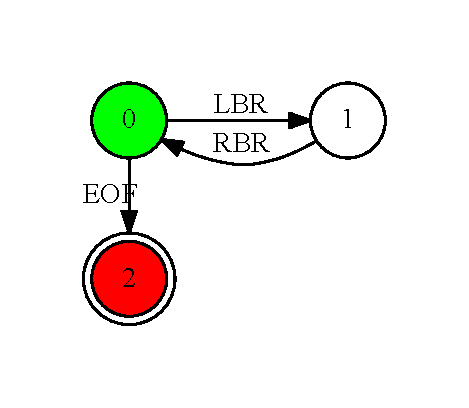
\includegraphics[width=2.5cm]{figures/in3.pdf}

            Грамматика:
            {\begin{align*}
                start& & &\Coloneq & &s \\
                s & & &\Coloneq & &\mbox{\texttt{LBR }} s \mbox{\texttt{ RBR }} s \\
                s & & &\Coloneq & &\varepsilon
            \end{align*}}
        \end{column}
        %\hspace{1cm}
        \begin{column}[T]{.6\textwidth}
            \vspace{-2em}
            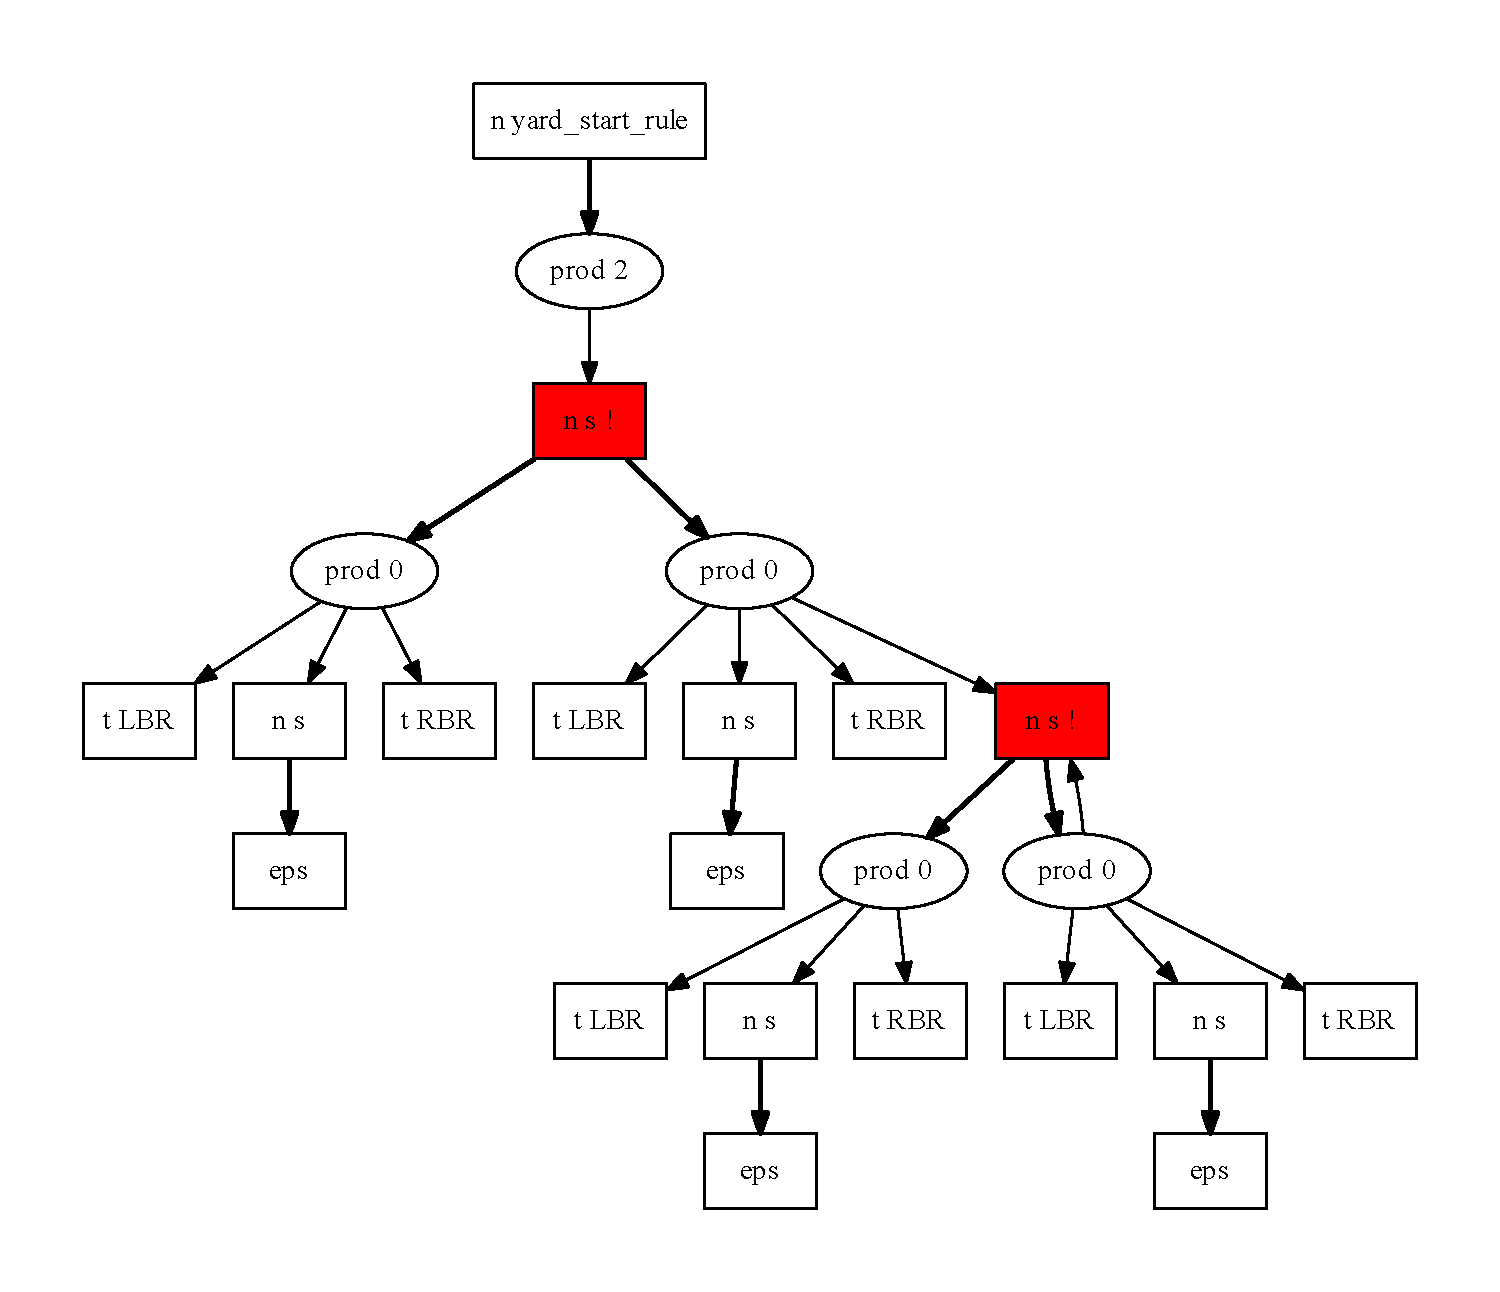
\includegraphics[width=1\textwidth]{figures/out3.pdf}
        \end{column}
    \end{columns}
\end{frame}

\begin{frame}
    \frametitle{Доказательство корректности алгоритма}
    {\small Формулировки утверждений. Идеи доказательств проговариваются устно.}
    \begin{rutheorem}[Пифагора: геометрическая формулировка]
        В прямоугольном треугольнике площадь квадрата, построенного на гипотенузе, равна сумме площадей квадратов, построенных на катетах.
    \end{rutheorem}

    \begin{rutheorem}[Пифагора: алгебраическая формулировка]
        В прямоугольном треугольнике квадрат длины гипотенузы равен сумме квадратов длин катетов.

        То есть, если обозначить длину гипотенузы треугольника через $c$, а длины катетов
        через $a$ и $b$, получим верное равенство: $a^2 + b^2 = c^2$.
    \end{rutheorem}

    \begin{rutheorem}[Обратная теорема Пифагора]
        Для всякой тройки положительных чисел $a$, $b$ и $c$, такой, что $a^2 + b^2 = c^2$, существует прямоугольный треугольник с катетами $a$ и $b$ и гипотенузой $c$.
    \end{rutheorem}
\end{frame}

\begin{frame}
    \frametitle{Архитектура решения}
    \begin{itemize}
        \item В реализации интересны архитектура, библиотеки, инструменты
        \item Не надо добавлять на слайд примеры кода
        \item Текст в квадратиках должен быть читаемым (крупным, а не как тут)
    \end{itemize}
    \begin{center}
        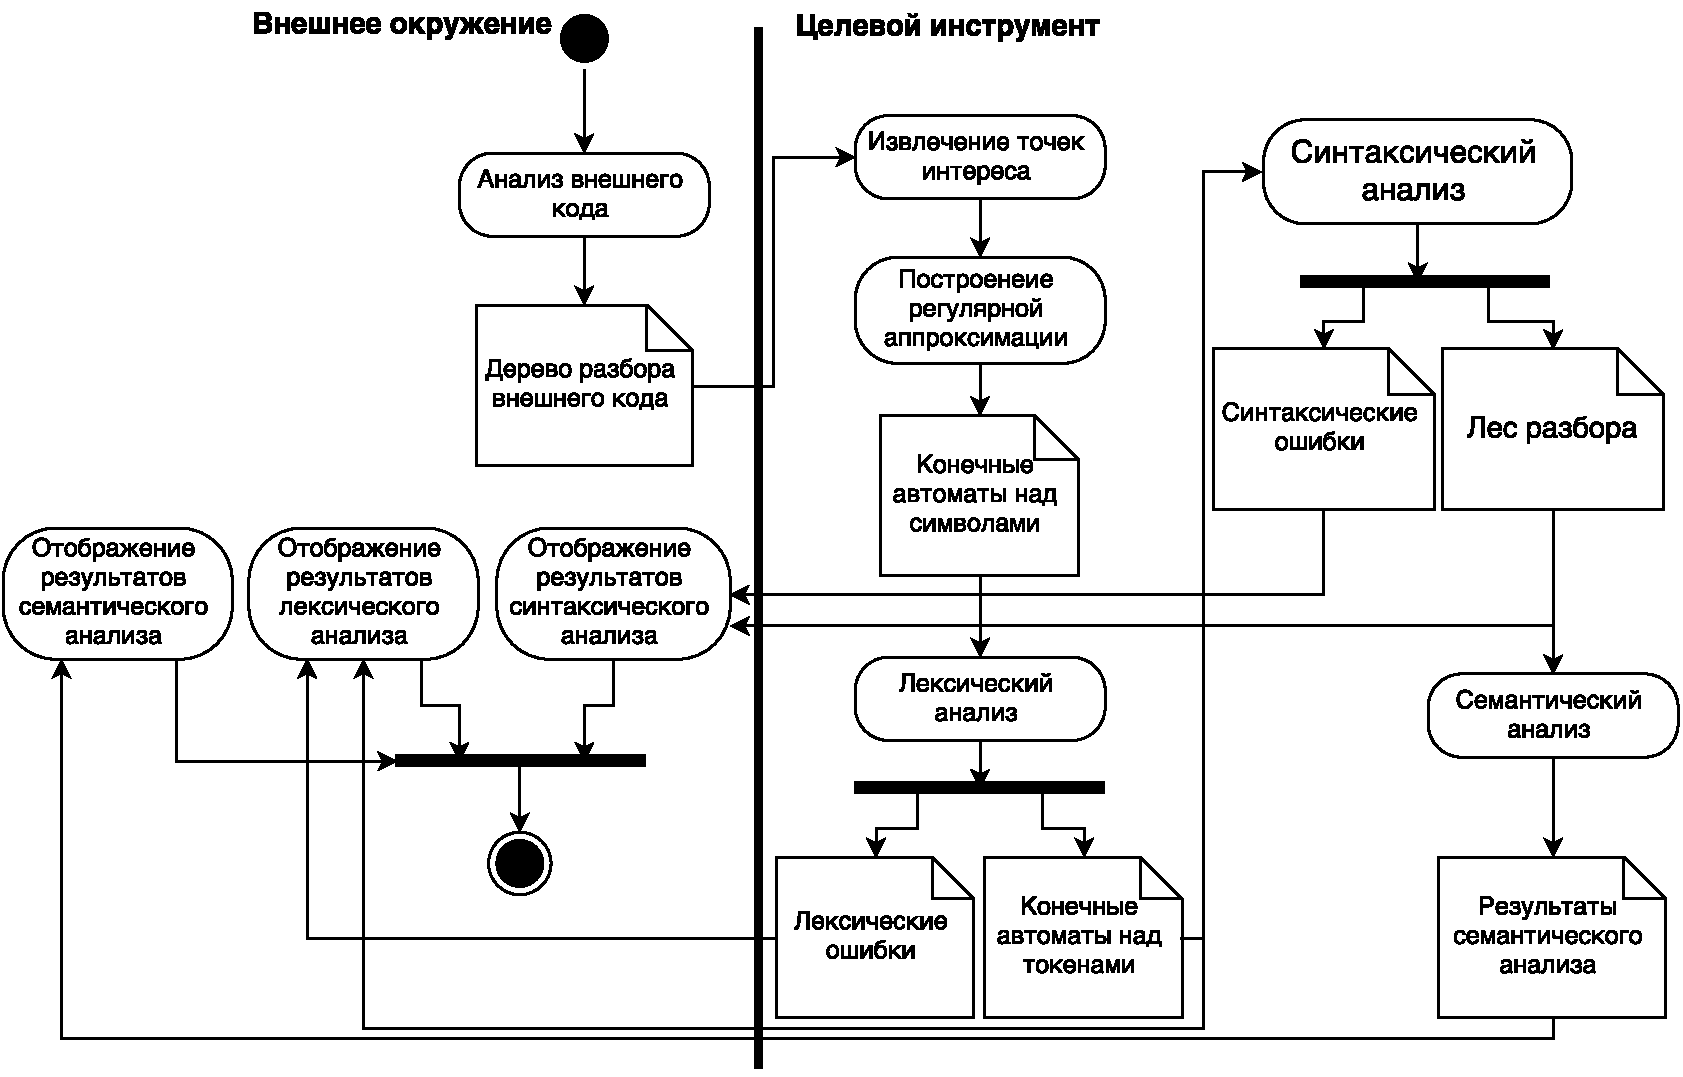
\includegraphics[width=0.7\textwidth]{figures/Activ_SEL_Processing.pdf}
    \end{center}
\end{frame}

\begin{frame}[t]
    \frametitle{Экспериментальное исследование}
    Постановка эксперимента
    \begin{itemize}
        \item На каком наборе данных проводилось экспериментальное исследование, почему были выбраны именно эти данные
        \item На каком оборудовании проводилось исследование
        \item Какие решения были выбраны для сравнения и почему
    \end{itemize}
\end{frame}

\begin{frame}[t]
    \frametitle{Результаты экспериментального исследования}
    \begin{itemize}
        \item Какие результаты показало экспериментальное исследование
        \item Желательно привести графики, иллюстрирующие полученные результаты
              \begin{itemize}
                  \item У иллюстраций должны быть подписи, у графиков~--- легенда, подписи к осям, например:
              \end{itemize}
    \end{itemize}
    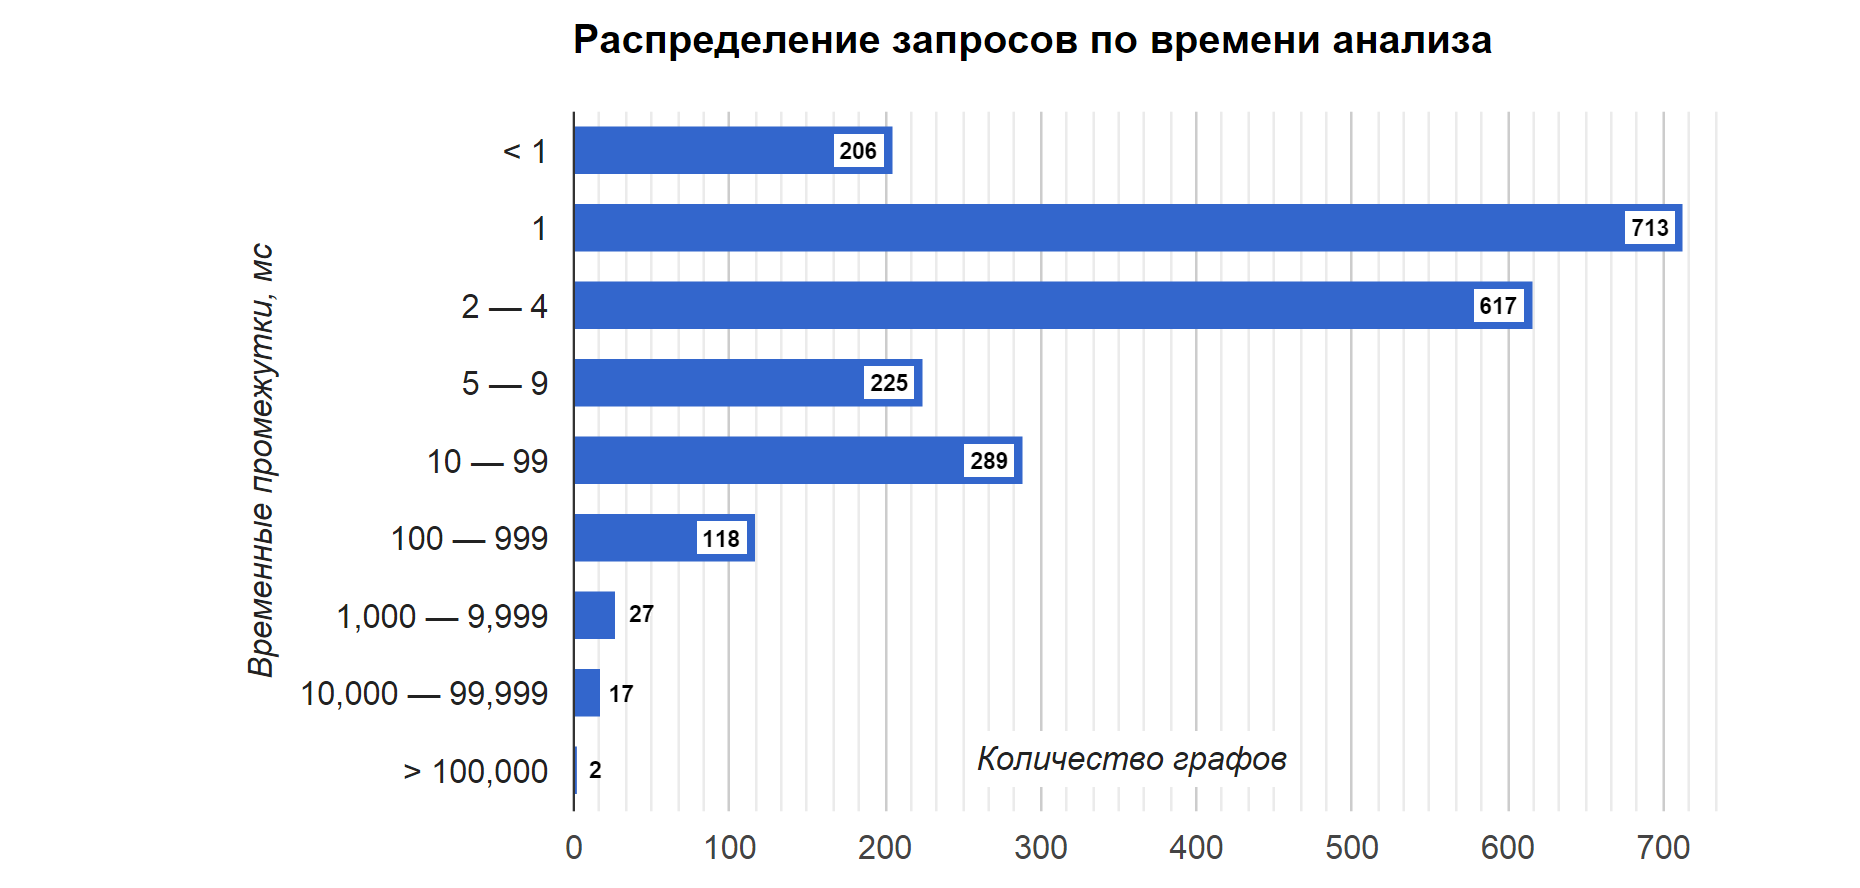
\includegraphics[width=13cm]{figures/dist.png}
\end{frame}

\begin{frame}
    \frametitle{Результаты}
    \begin{itemize}
        \item Практически то же, что и на слайде с постановкой задачи, но в совершенной форме~--- что делал лично автор
        \item Четкое отделение результатов своей работы (особенно для коллективных работ)
        \item Формулировать глаголами совершенного вида в прошедшем времени (\enquote{сделано}, \enquote{получено})
        \item Обсуждение (ограничения, валидность, альтернативы)
        \item Не нужно слайдов типа \enquote{Все}, \enquote{Вопросы?}, \enquote{Спасибо за внимание}
    \end{itemize}

    \begin{itemize}
        \item Если результаты были представлены на конференции и опубликованы, это желательно указать
    \end{itemize}
\end{frame}

%\addtocounter{framenumber}{1}
\appendix

\begin{frame}
    \frametitle{Дополнительный слайд}
    Например, с огромной страшной формулой всего, которая нужна для пояснения деталей при ответе на частый вопрос

    \begin{align*}
        \MoveEqLeft \lim_{\bigtriangleup t \to 0^+}\int_{\bigtriangleup t}^{T} \! \int_{\Omega} \! D(t_1,x) \frac{\varphi(t_1-\bigtriangleup t,x)-\varphi(t_1,x)}{(-\bigtriangleup t)} \, \mathrm{d}x \, \mathrm{d}t_1 \\
        &= \lim_{\bigtriangleup t \to 0^+} \int_{0}^{T} \! \int_{\Omega} \! D(t_1,x) \frac{\varphi(t_1-\bigtriangleup t,x)-\varphi(t_1,x)}{(-\bigtriangleup t)} \chi_{(\bigtriangleup t,T)}(t_1) \, \mathrm{d}x \, \mathrm{d}t_1 \\
        &=\int_{0}^{T} \! \int_{\Omega} \! D(t_1,x) \frac{\partial \varphi}{\partial t_1} (t_1,x) \, \mathrm{d}x \, \mathrm{d}t_1
    \end{align*}
\end{frame}

\begin{frame}
    \frametitle{Второй дополнительный слайд}
    \begin{itemize}
        \item Много дополнительных слайдов не надо: 1--2~вполне достаточно в большинстве случаев
        \item Кроме формул здесь могут быть схемы, рисунки, таблицы и другие вспомогательные материалы
    \end{itemize}

\end{frame}

\end{document}
